\documentclass{article}
\usepackage[margin=1in]{geometry}
\usepackage{longtable}
\usepackage{bm}
\usepackage{hyperref}
\hypersetup{
    colorlinks=true,
    linkcolor=black,
    filecolor=magenta,      
    urlcolor=red,
    citecolor=cyan
}
\usepackage{graphicx}
\usepackage{amsmath}
\usepackage{setspace}

\usepackage{amssymb}
\usepackage{natbib}
\usepackage{amsfonts}
\usepackage[table]{xcolor}
\usepackage{booktabs}
\usepackage{courier}

\newcommand\citeapos[1]{\citeauthor{#1}'s (\citeyear{#1})}

\begin{document}

\title{The Network of Foreign Direct Investment Flows: \\Theory and Empirical Analysis}
\author{John  Schoeneman\thanks{\footnotesize{
jbs5686@psu.edu, PhD Student, Pennsylvania State University.}} \and Boliang Zhu\thanks{\footnotesize{bxz14@psu.edu, Assistant Professor, Department of Political Science, Pennsylvania State University. }} \and Bruce A. Desmarais\thanks{\footnotesize{
bdesmarais@psu.edu, Associate Professor, Department of Political Science, Pennsylvania State University.}}}
\date{}
\maketitle

\singlespacing
\begin{abstract} 
    \noindent We study the structure of the international network of foreign direct investment (FDI) flows. The political economy of FDI literature has established several theoretical claims and empirical regularities regarding exogenous political and economic determinants of FDI inflows. These include security alliances, preferential trade agreements, migration networks, and colonial history. However, existing studies---based on monadic and to a lesser degree, dyadic regression models---overlook the complex dependencies that are likely to characterize the network. Recent developments in methodology for studying international relations show that the regression framework is typically inadequate for quantitatively modeling dyadic relational data, such as FDI flows. In this paper, we integrate hypotheses regarding exogenous determinants and novel hypotheses regarding structural dependencies into a comprehensive exponential random graph model (ERGM) for weighted networks. Our findings reveal that the FDI flow network  exhibits a number of complex dependencies, such as reciprocity, that have been omitted from previous empirical models of FDI flows.

\end{abstract}

\section{Introduction}

Research examining foreign direct investment (FDI) and its relationship with economic and political determinants is expansive. Much of this work is conducted using the gravity model, which was originally developed to predict trade flows. This framework models FDI flows using dyadic data and the product of partner GDPs as mass and some variant of distance as an independent variable. Our work highlights a key weakness of these models that rely on standard panel regression models. There has been a growing body of literature that brings into question the way we estimate models for dyadic data. The primary challenge is that dyadic data is an edge-list and therefore represents a network. Ignoring this unmodeled network structure violates assumptions within a generalized linear model, particularly independence, potentially leading to biased estimates. While there is a growing body of work that has addressed the interdependence problem in dyadic data, especially for trade, FDI has been largely ignored. We address this gap in the literature through the use of network modeling to test previous theories alongside of estimating dependence terms.


{\bf [John or Boliang, paragraph on what scholars have asked or know about FDI]}



\section{Independence Assumptions and the study of FDI}

Paragraph on the focus of quantitative models of FDI, emphasizing that scholars typically assume that flows arise independently {\bf [Boliang]}.

% Paragraph on interdependence in IR/IPE
Historically, statistical models used in international relations have involved the implicit assumption that countries and dyads are independent of each other \citep{diehl2016conditional,ward2007persistent}. This assumption is now widely viewed as dubious \citep[see, e.g., ][]{ward2007persistent, chu2010homogenization,cranmer2016critique,dorff2013networks,lee2013network,howell2013geography,kinne2016agreeing}. The negative consequences of erroneously assuming independence are two-fold. First, the model is misspecified, which leads to biased estimates and hypothesis tests for covariates included in the model. Second, researchers arrive at a limited theoretical scope in which they only consider the relationship between the dependent variable and covariates, and do not consider the influences that relationships and countries have on each other. The methodological toolkit available to scholars of international relations has advanced well beyond conventional regression approaches, and now offers at least three prominent options for modeling interdependence in relational data----stochastic actor oriented models \citep[e.g., ][]{camber2010geometry,kinne2016agreeing,kinne2013network,kinne2014dependent,warren2016modeling}, exponential random graph models \citep[e.g.,][]{cranmer2012complex,cranmer2012toward,raeymaeckers2016influence}, and latent space models \citep[e.g., ][]{ward2007disputes,ward2013gravity,metternich2013antigovernment}. As such, it is quite methodologically feasible to move beyond questionable independence assumptions in the study of FDI.

\section{Dependence Hypotheses in FDI Flows}

Scholars have long been interested in understanding investment flows across countries. Standard economic models attribute cross-border capital movements primarily to relative factor endowments, market size, and transportation and trade cost \citep[see,~e.g.,][]{Helpman:1984,Carr_et_al:2001}. Yet, footloose capital becomes immobile ex post and thus an ``obsolescent bargain,'' which is vulnerable to host government's expropriation \citep{Vernon:1971,Vernon:1980}. Building on this insight, the recent political economy of FDI literature emphasizes the importance of political institutions in constraining host government's opportunistic behavior. Scholars suggest that political constraints \citep{Henisz:2000}, democratic governance \citep{Jensen:2003,Jensen:2006}, rule of law \citep{Li_Resnick:2003,Staats_Biglaiser:2012}, and participation in international institutions \citep{Buthe_Milner:2008,Allee_Peinhardt:2011} help to ensure policy credibility and provide investor protection, thereby luring in foreign investors.

There is now a large empirical literature examining the determinants of FDI inflows \citep[e.g.,][]{Noorbakhsh_et_al:2001,Yeaple:2003,Jensen:2003,Li_Resnick:2003,Buthe_Milner:2008,Li_Vashchilko:2010,Kerner:2009}. Existing studies typically model FDI flows at the monadic or dyadic level. One crucial assumption in these models is that FDI flows into one country or between one dyad are independent of other countries or dyads. This assumption, nonetheless, unlikely holds, given the intertwined links among MNCs and the expansion of global production networks. If global FDI flows can arise endogenously from its network structure, existing political economy models of FDI remain incomplete by excluding structural variables. Moreover, ignoring the network dependencies of FDI flows can result in biased estimates or even invalid inferences \citep{Cranmer_Desmarais:2011}. To the best of our knowledge, no existing research has systematically examined network dependencies of global FDI flows. We seek to bridge this gap in the paper. We expect two network structures---reciprocity and transitivity---are important to account for the pattern of cross-border FDI flows.

\subsection{Reciprocity of FDI Flows}
Reciprocity stems from the fact that FDI represents an oligopolistic expansion strategy of MNCs \citep{Hymer:1976,Kindleberger:1969}. MNCs arise from exploiting their ownership-specific assets to overcome imperfections in arm's-length markets \citep{Caves:1996,Dunning:1002}. These proprietary assets include, for instance, advanced technology, brand names, product differentiation, and managerial and advertising skills, which are of a public-goods character and possess substantial economies of scale. To make the most use of these firm-specific assets and best exploit economies of scale, MNCs actively seek to expand into each other's home markets. Unsurprisingly, until the first decade of the new century FDI flows mainly between developed countries, especially among the triad of the European Union, Japan, and the United States.

MNCs' oligopolistic expansion often encounters opposition from host government for the sake of national security, market competition, and protection of indigenous firms. In order to gain access to foreign markets, MNCs have incentives to leverage their influence on home government for reciprocity \citep{Milner:1988,Crystal:2003}. As \citet[6]{Crystal:2003} note, ``they [MNCs] want to counter the existing restrictions---on both trade and FDI---that some foreign countries have imposed and so therefore will favor contingently restrictive policies.'' \citet{Tingley:2015}, for instance, show that U.S. government officials are more likely to oppose Chinese firms' mergers and acquisitions when China has blocked U.S. investment.

We also expect that the degree of reciprocity varies by host countries' levels of development. Investing abroad incurs large fixed costs and firms need to overcome the disadvantages such as ``liability of foreignness'' they face when competing with indigenous firms in the host country. Therefore, only the most productive firms are able to engage in FDI activities \citep{Melitz:2003,Helpman_et_al:2004}. Historically, MNCs from developed countries predominate. In the past two decades, FDI from developing and transition economies have grown rapidly. Yet developing-country MNCs still account for a relatively small share of global outward FDI. For instance, in 2005 outward FDI flows and stocks from developing countries are approximately 17\% and 13\% of the world total, respectively \citep{UNCTAD:2006}. Furthermore, outward FDI from developing countries is highly concentrated; the top 10 countries, mostly large emerging economies such as Argentina, Brazil, Chile, China, Mexico, Russia, and South Africa contribute about 83\% \citep{UNCTAD:2006}. Firms in most developing countries are still technologically backward and not competitive enough to strive in a global market. Thus, we hypothesize the following:

\textit{Hypothesis 1: FDI flows are likely to be reciprocal.}

\textit{Hypothesis 1a: The reciprocity of FDI flows is stronger among developed dyads than others.}

\subsection{Transitivity/Clustering of FDI Flows}
Two factors are likely to drive the transitivity/clustering of investment activities---the expansion of global supply chains and the diffuse of preferential trade agreements (PTAs).  One distinct feature of today's globalization is the increasing fragmentation of production processes and the dramatic expansion of global supply chains \citep{UNCTAD:2013}. At the center of global production networks are MNCs, which coordinate global supply chains through complex networks of their foreign affiliates, subcontractors, or arm's-length suppliers \citep[xxii]{UNCTAD:2013}. These intertwined networks give rise to the clustering of FDI activities. In a most straightforward way, MNCs' establishment of a foreign affiliate is typically followed by investment of their partners such as upstream customers or downstream suppliers, who themselves are often multinationals that coordinate their own networks of supply chains. This kind of interdependent linkages lead to multiple triangle closures of investment flows. Consider a case of three countries: A, B, and C. Firms from A invest in B as suppliers to firms in B.\footnote{Alternatively, firms in A can export intermediate goods to B. However, firms typically favor near suppliers. Moreover, if transportation and trade costs between A and B are high, firms in A will prefer direct investment over export \citep{Carr_et_al:2001}. } If firms in B establish foreign affiliates in C to exploit locational advantages, investment by firms in A likely follows to serve these foreign affiliates. [Need a real example, e.g. automotive industry FDI]

More importantly, global supply chains tie countries together and significantly increase the cost of government's opportunistic behavior---such as expropriation or subtle policy changes---that deters foreign investment. Investors' wariness stems from the fact that footloose capital becomes an ``obsolescent bargain'' given its ex post immobility, and thus a hostage to the host government \citep{Vernon:1971,Vernon:1980}. Global production networks significantly constraint government's policy discretion, because the proper functioning of the supply chains hinges crucially on the cooperation and coordination of countries involved. For example, even Starbucks, a company that has a relatively simple supply chain, ``sources coffee from thousands of traders, agents and contract farmers across the developing world; manufactures coffee in over 30 plants, ...; distributes the coffee to retail outlets through over 50 major central and regional warehouses and distribution centres; and operates some 17,000 retail stores in over 50 countries across the globe'' \citep[142]{UNCTAD:2013}. 

Apparently, any interruption in the global supply chain can severely damage Starbucks's business. Thus, governments are incentivized to refrain from arbitrary interventions or even subtle policy changes that dampen firms' profitability. Especially when countries are integrated into the same global production network, the risk-mitigating effect of the network is magnified because involving countries have strong incentives to ensure the well-functioning of the network, on which their fortunes depend. As \citet{Kim_Solingen:2017} show, East Asian countries that are deeply integrated into global production networks are more likely to promote cooperation and peace between each other. Therefore, we expect that FDI has a higher probability than a random chance to flow among countries that are in the same global production network, resulting in the clustering of investment activities.

The clustering of direct investment activities can be driven by the diffuse of PTAs as well. The formation of a PTA eliminates trade barriers among member states. The removal of trade barriers allows MNCs to optimize their global supply chains and fragment its production stages within member states to best capitalize on locational advantages such as factor endowments and favorable government policies. For instance, with the increasing integration of the European Community, the 1980s witnessed a restructuring of many industries and regionalization of MNC activities to exploit the advantages of a single market, leading to a surge of intra-region FDI \citep[34]{UNCTAD:1991}. Importantly, most favored-nation treatment, investment clauses, and dispute-settle mechanisms that are embedded in PTAs help to alleviate foreign investors' concerns of government interventions, discrimination, and expropriation \citep{Buthe_Milner:2008,buthe2014foreign}, thereby making member states more attractive investment destinations for each other. PTAs therefore reinforce the clustering of investment activities.

\textit{Hypothesis 2: FDI flows are likely to be transitive/clustering.}




\section{Data and Research Design}

\subsection{The Count ERGM for Modeling FDI Networks}

To model the FDI network, we must use a statistical modeling approach that is capable of representing the dependencies underlying the ties. The literature offers a number of options. These include the latent space family of models, such as those that have been used to model trade networks in political science \citep{ward2007persistent,ward2013gravity}; the generalized exponential random graph model (GERGM), which can be used to model complex network features in networks with continuous-valued edges \citep{desmarais2012statistical,wilson2017stochastic}; and the ERGM for count-valued edges \citep{krivitsky2012exponential}. We select the count-valued ERGM for two reasons. First, if the researcher's objective is to test hypotheses regarding dependent network structure, ERGM family models can accomplish this more precisely than can latent space models \citep{cranmer2016navigating,cranmer2016critique,desmarais2017statistical}. Second, the count ERGM offers a modeling advantage over the GERGM for data such as FDI flows, which are zero for the majority of dyads. That is, the count ERGM is capable of modeling zero inflation in the network. This paper presents, as far as we are aware, the first application in political science of the count ERGM proposed by \cite{krivitsky2012exponential}.

Like other forms of the ERGM, the count ERGM is a statistical model that operates on one or more network adjacency matrices. To specify the count ERGM, the researcher selects two types of network statistics---those that relate tie values to observed covariates (i.e., covariate effects), and those that relate the ties to each other via high order network structure (i.e., network effects). If an ERGM is specified without network effects, it reduces to a dyadic regression model in which ties are assumed to be independent and identically distributed \cite{cranmer2011inferential}. Under \citeapos{krivitsky2012exponential} count ERGM, the probability of the observed $n \times n$ network adjacency matrix $\bm{y}$ is $$ \text{Pr}_{\bm{\theta};h;\bm{g}}( \bm{Y}=\bm{y} )=\frac{ h(\bm{y})\text{exp}( \bm{\theta} \cdot \bm{g} (\bm{y}) )}{\bm{\kappa}_{h,\bm{g}}(\bm{\theta})},$$ where $\bm{g}( \bm{y} )$ is the vector of network statistics used to specify the model, $bm{\theta}$ is the vector of parameters that describes how those statistic values relate to the probability of observing the network, $h(\bm{y})$ is a reference function defined on the support of $\bm{y}$ and selected to affect the shape of the baseline distribution of dyadic data (e.g., Poisson reference measure), and $\bm{\kappa}_{h,\bm{g}}(\bm{\theta})$ is the normalizing constant that assures that the probabilities over all possible networks sums to one. 






\subsection{FDI inflows}

For the dependent variable we are using bilateral FDI inflows. These are from the United Nations Conference on Trade and Development (UNCTAD) and were first made available in 2014 \citep{UNCTAD}. We use the entire time-period available, which is 2001-2012. Past work that has looked at country-year FDI relationships relied on monadic data. The advantage of using dyadic data is that it not only lets us model network relationships, but the disaggregation allows us to measure changes in FDI inflows related to covariates that are at the dyad level, such as PTAs. Because FDI flows tend to be highly dispersed we use the natural log of the values. 

\subsection{Network Statistics}

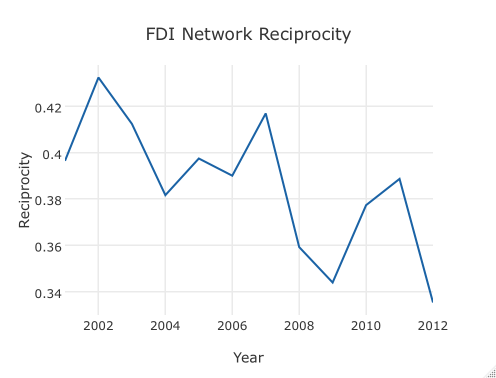
\includegraphics[scale=.8]{draft_figures/reciprocity.png}\\
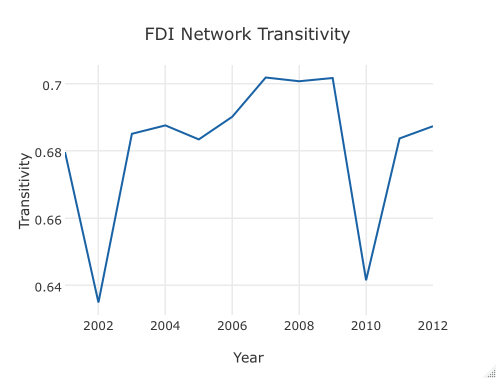
\includegraphics[scale=.8]{draft_figures/transitivity.png}\\
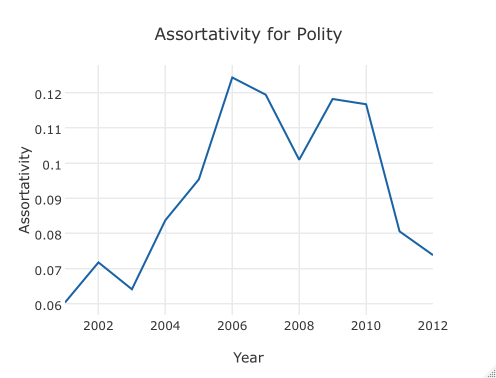
\includegraphics[scale=.8]{draft_figures/assortativity.png}\\
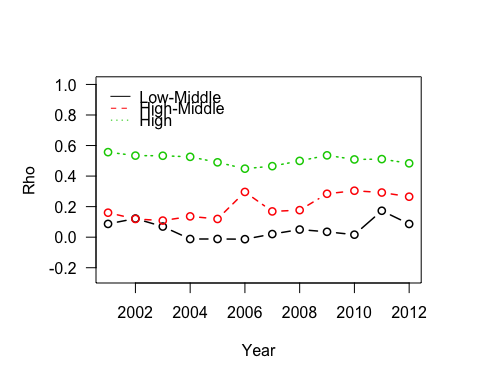
\includegraphics[scale=.8]{draft_figures/rho_income.png}\\
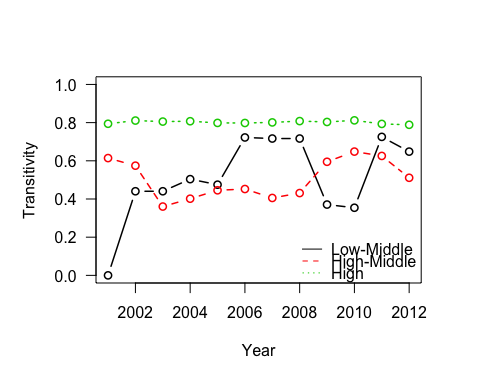
\includegraphics[scale=.8]{draft_figures/trans_income.png}\\
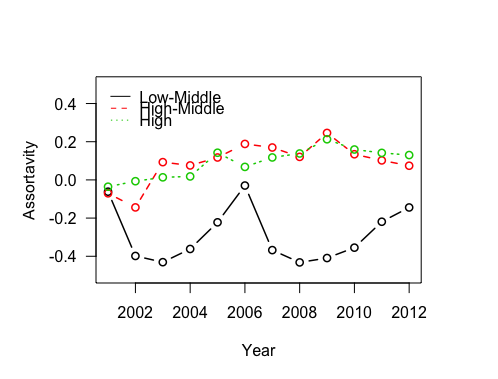
\includegraphics[scale=.8]{draft_figures/assort_income.png}

\subsection{Covariates}

We control for both economic and political variables. Following the literature's standard for predicting FDI inflows we include standard gravity variables. This includes the log product of the dyad's GDP and logged euclidean distance. Generally, larger products of GDP are associated with higher levels of FDI while longer distances are associated with less FDI \citep{mayer2011notes, WB1}. \\

The other key economic variable that is included trade in intermediate goods \citep{OECD}. This is constructed according to the UN Broad Economic Category classification definitions that separates goods by end-use category. Intermediate goods include unprocessed and partially processed agricultural goods and industrial goods. Past research has shown that FDI and trade are compliments \citep{aizenman2006fdi} and the advantage of using trade in intermediate goods is that it proxies for production supply chains, which we expect to be strongly positively associated with FDI inflows.\\

A more minor economic variable included is the growth rate of the economy, which has been used in past studies to stand in for the general health of a country's economy \citep{WB2}.\\

We include two categories of international agreement variables. The first is dummy variables for defense agreements \citep{Gibler09}. This includes defense, entente, non-aggression, and neutrality treaties. We expect these variables to positively associated with FDI inflows, particularly defense treaties since this indicates political cooperation and a lower risk of expropriation. The second international agreement variable is preferential trade agreement (PTA) depth \citep{dur2014design}. Past work has argued that PTAs represent a commitment to liberal markets that investors would favor and therefore would be associated with increased FDI inflows \citep{buthe2014foreign}. However, this study used monadic data and only a count PTAs signed. Our work takes this further since we are using network data and increases in PTA depth and FDI inflows is measured at the dyadic level and the PTA variable we use is built using latent trait analysis with 48 different variables.\\

There is substantial amount of work that explores the relationship between regime type and FDI inflows. The work is inconclusive, but include controls for it nonetheless using the Polity IV score \citep{polity2012polity}. We also include political violence to proxy for state stability, which expect to be negatively correlated with FDI inflows \citep{marshall2005major}.

\subsection{Model Specification}
The count ERGM is extremely flexible in that there are very few constraints on the generative features that can be incorporated into the model through $\bm{g}( \bm{y} )$. In the models we specify, we use statistics that model the shape of the individual edge distributions (i.e., the shapes of directed dyadic FDI flows), model the dependencies we have described above, and account for the effects of exogenous covariates. The statistics we use to account for the individual edge distribution include, $$\text{Sum}:\bm{g(y)} = \sum_{(i,j) {\in} \mathbb{Y}}\bm{y}_{i,j},$$ which models the average edge value $$\text{Sum, Fractional Moment}:\bm{g(y)} = \sum_{(i,j) {\in} \mathbb{Y}}\bm{y}_{i,j}^{1/2},$$ which accounts for dispersion in the edge distribution, and
$$\text{Non-Zero}: \bm{g}_k = \sum_{(i,j) {\in} \mathbb{Y}} \mathbb{I}(\bm{y}_{i,j} \neq 0),$$ which models the prevalence of zeros in dyadic FDI flows. We include two statistics to model the dependencies that correspond to our hypotheses. First,
$$ \text{Reciprocity}: \bm{g(y)} = \sum_{(i,j) {\in} \mathbb{Y}}min(\bm{y}_{i,j},\bm{y}_{j,i}),$$ in which we add up the lowest edge value within each dyad. If edges are reciprocated, this statistic will increase due to the co-occurrence of large edge values within the same dyad. Second, 
$$\text{Transitive Weights}: \bm{g(y)} =  \sum_{(i,j) {\in} \mathbb{Y}}\min\bigg( \bm{y}_{i,j}, \max\limits_{k{\in}N}\Big(\min(\bm{y}_{i,k},\bm{y}_{k,j})\Big) \bigg),$$ which acounts for the degree to which edge $(i,j)$ co-occurs with pairs of large edge values with which  edge $(i,j)$ forms a transitive (i.e., non-cyclical) triangle. Exogenous covariates are accounted for with statistics that measure the degree to which large covariate values co-occur with large edge values. First,
$$ \text{Dyadic Covariate}: \bm{g(y,x)} = \sum_{(i,j)} \bm{y}_{i,j}x_{i,j},$$ measures this co-occurrence at the level of the directed dyad, in which there is a dyadic observation of the covariate corresponding to each potential FDI flow. There are two statistics that account for node (i.e., country) level covariates. Each statistic takes the product of the node's covariate value and a sum of the edge values in which the node is involved. The first, ``Sender Covariate,'' uses the sum over the flows that the node sends. The second, ``Receiver Covariate,'' uses the sum over the flows that the node receives. These two variants of node-level statistics differentiate between the effects of a variable on the volume of FDI originating from a state, and being invested in a state, respectively.

$$ \text{Sender Covariate}: \bm{g(y,x)} = \sum_{i}x_i \sum_{j} \bm{y}_{i,j}$$

$$ \text{Receiver Covariate}: \bm{g(y,x)} = \sum_{j}x_j \sum_{i} \bm{y}_{i,j}$$

\subsection{Covariate Summary Statistics}

% Table created by stargazer v.5.2 by Marek Hlavac, Harvard University. E-mail: hlavac at fas.harvard.edu
% Date and time: Mon, Feb 20, 2017 - 22:08:59
\begin{table}[!htbp] \centering 
  \caption{} 
  \label{} 
\begin{tabular}{@{\extracolsep{5pt}}lccccc} 
\\[-1.8ex]\hline 
\hline \\[-1.8ex] 
Statistic & \multicolumn{1}{c}{N} & \multicolumn{1}{c}{Mean} & \multicolumn{1}{c}{St. Dev.} & \multicolumn{1}{c}{Min} & \multicolumn{1}{c}{Max} \\ 
\hline \\[-1.8ex] 
Contiguity & 189,000 & 0.024 & 0.152 & 0 & 1 \\ 
Common Official Language & 189,000 & 0.112 & 0.315 & 0 & 1 \\ 
Common Language and Ethnicity & 189,000 & 0.115 & 0.318 & 0 & 1 \\ 
Former Colonial Relationship & 189,000 & 0.015 & 0.121 & 0 & 1 \\ 
Common Colonizer & 189,000 & 0.062 & 0.241 & 0 & 1 \\ 
Defense Treaty & 189,000 & 0.075 & 0.264 & 0 & 1 \\ 
Non-aggression Treaty & 189,000 & 0.064 & 0.245 & 0 & 1 \\ 
Neutrality Treaty & 189,000 & 0.004 & 0.063 & 0 & 1 \\ 
Entente Treaty & 189,000 & 0.066 & 0.248 & 0 & 1 \\ 
\hline \\[-1.8ex] 
\end{tabular} 
\end{table} 



\newpage
\begin{table}[!htbp] \centering 
  \caption{Year 2007} 
  \label{} 
\small 
\begin{tabular}{@{\extracolsep{2pt}}lcc} 
\\[-1.8ex]\hline 
\hline \\[-1.8ex] 
 & \multicolumn{2}{c}{\textit{Dependent variable:}} \\ 
\cline{2-3} 
\\[-1.8ex] & \multicolumn{2}{c}{fdi\_net} \\ 
\\[-1.8ex] & (1) & (2)\\ 
\hline \\[-1.8ex] 
 sum & $-$4.008$^{***}$ & $-$3.984$^{***}$ \\ 
  & (0.203) & (0.209) \\ 
  sum0.5 & 15.231$^{***}$ & 13.695$^{***}$ \\ 
  & (0.457) & (0.458) \\ 
  nonzero & $-$16.176$^{***}$ & $-$14.982$^{***}$ \\ 
  & (0.376) & (0.364) \\ 
  mutual.min &  & 0.179$^{***}$ \\ 
  &  & (0.035) \\ 
  transitiveweights.min.max.min &  & 0.724$^{***}$ \\ 
  &  & (0.052) \\ 
  edgecov.fdi\_net.lag\_stock.sum & 0.376$^{***}$ & 0.372$^{***}$ \\ 
  & (0.009) & (0.009) \\ 
  edgecov.fdi\_net.mass.sum & 1.516$^{***}$ & 0.934$^{***}$ \\ 
  & (0.096) & (0.105) \\ 
  edgecov.fdi\_net.distance.sum & $-$0.129$^{***}$ & $-$0.114$^{***}$ \\ 
  & (0.014) & (0.016) \\ 
  edgecov.fdi\_net.contig.sum & $-$0.116$^{**}$ & $-$0.066 \\ 
  & (0.051) & (0.056) \\ 
  edgecov.fdi\_net.colony.sum & $-$0.054 & $-$0.103$^{*}$ \\ 
  & (0.053) & (0.055) \\ 
  edgecov.fdi\_net.lang\_ethno.sum & 0.081$^{**}$ & 0.074$^{**}$ \\ 
  & (0.033) & (0.034) \\ 
  edgecov.fdi\_net.defence\_t.sum & $-$0.044 & 0.044 \\ 
  & (0.082) & (0.090) \\ 
  edgecov.fdi\_net.nonagg\_t.sum & $-$0.040 & $-$0.068 \\ 
  & (0.093) & (0.098) \\ 
  edgecov.fdi\_net.neut\_t.sum & 0.312$^{***}$ & 0.407$^{***}$ \\ 
  & (0.105) & (0.118) \\ 
  edgecov.fdi\_net.entente\_t.sum & $-$0.045 & $-$0.088 \\ 
  & (0.100) & (0.109) \\ 
  edgecov.fdi\_net.depth.sum & 0.115$^{***}$ & 0.080$^{**}$ \\ 
  & (0.041) & (0.041) \\ 
  nodeocov.sum..Polity & 0.198$^{***}$ & 0.122$^{***}$ \\ 
  & (0.044) & (0.042) \\ 
  nodeocov.sum..TradeOpen & 0.307$^{***}$ & 0.183$^{**}$ \\ 
  & (0.069) & (0.071) \\ 
  nodeocov.sum..GDP.g & $-$0.058 & 0.011 \\ 
  & (0.099) & (0.100) \\ 
  nodeocov.sum..PV & $-$0.023 & 0.048 \\ 
  & (0.064) & (0.066) \\ 
  nodeocov.sum..GDPpc & 0.549$^{***}$ & 0.504$^{***}$ \\ 
  & (0.068) & (0.075) \\ 
  nodeicov.sum..Polity & 0.051 & $-$0.027 \\ 
  & (0.040) & (0.040) \\ 
  nodeicov.sum..TradeOpen & 0.287$^{***}$ & 0.164$^{*}$ \\ 
  & (0.078) & (0.086) \\ 
  nodeicov.sum..GDP.g & $-$0.236$^{**}$ & $-$0.112 \\ 
  & (0.096) & (0.093) \\ 
  nodeicov.sum..PV & $-$0.125$^{*}$ & $-$0.067 \\ 
  & (0.069) & (0.077) \\ 
  nodeicov.sum..GDPpc & $-$0.250$^{***}$ & $-$0.474$^{***}$ \\ 
  & (0.090) & (0.093) \\ 
 \hline \\[-1.8ex] 
Akaike Inf. Crit. & $-$42,994.640 & $-$40,831.300 \\ 
Bayesian Inf. Crit. & $-$42,811.080 & $-$40,632.430 \\ 
\hline 
\hline \\[-1.8ex] 
\textit{Note:}  & \multicolumn{2}{r}{$^{*}$p$<$0.1; $^{**}$p$<$0.05; $^{***}$p$<$0.01} \\ 
\end{tabular} 
\end{table} 

\begin{figure}[h]
\centering
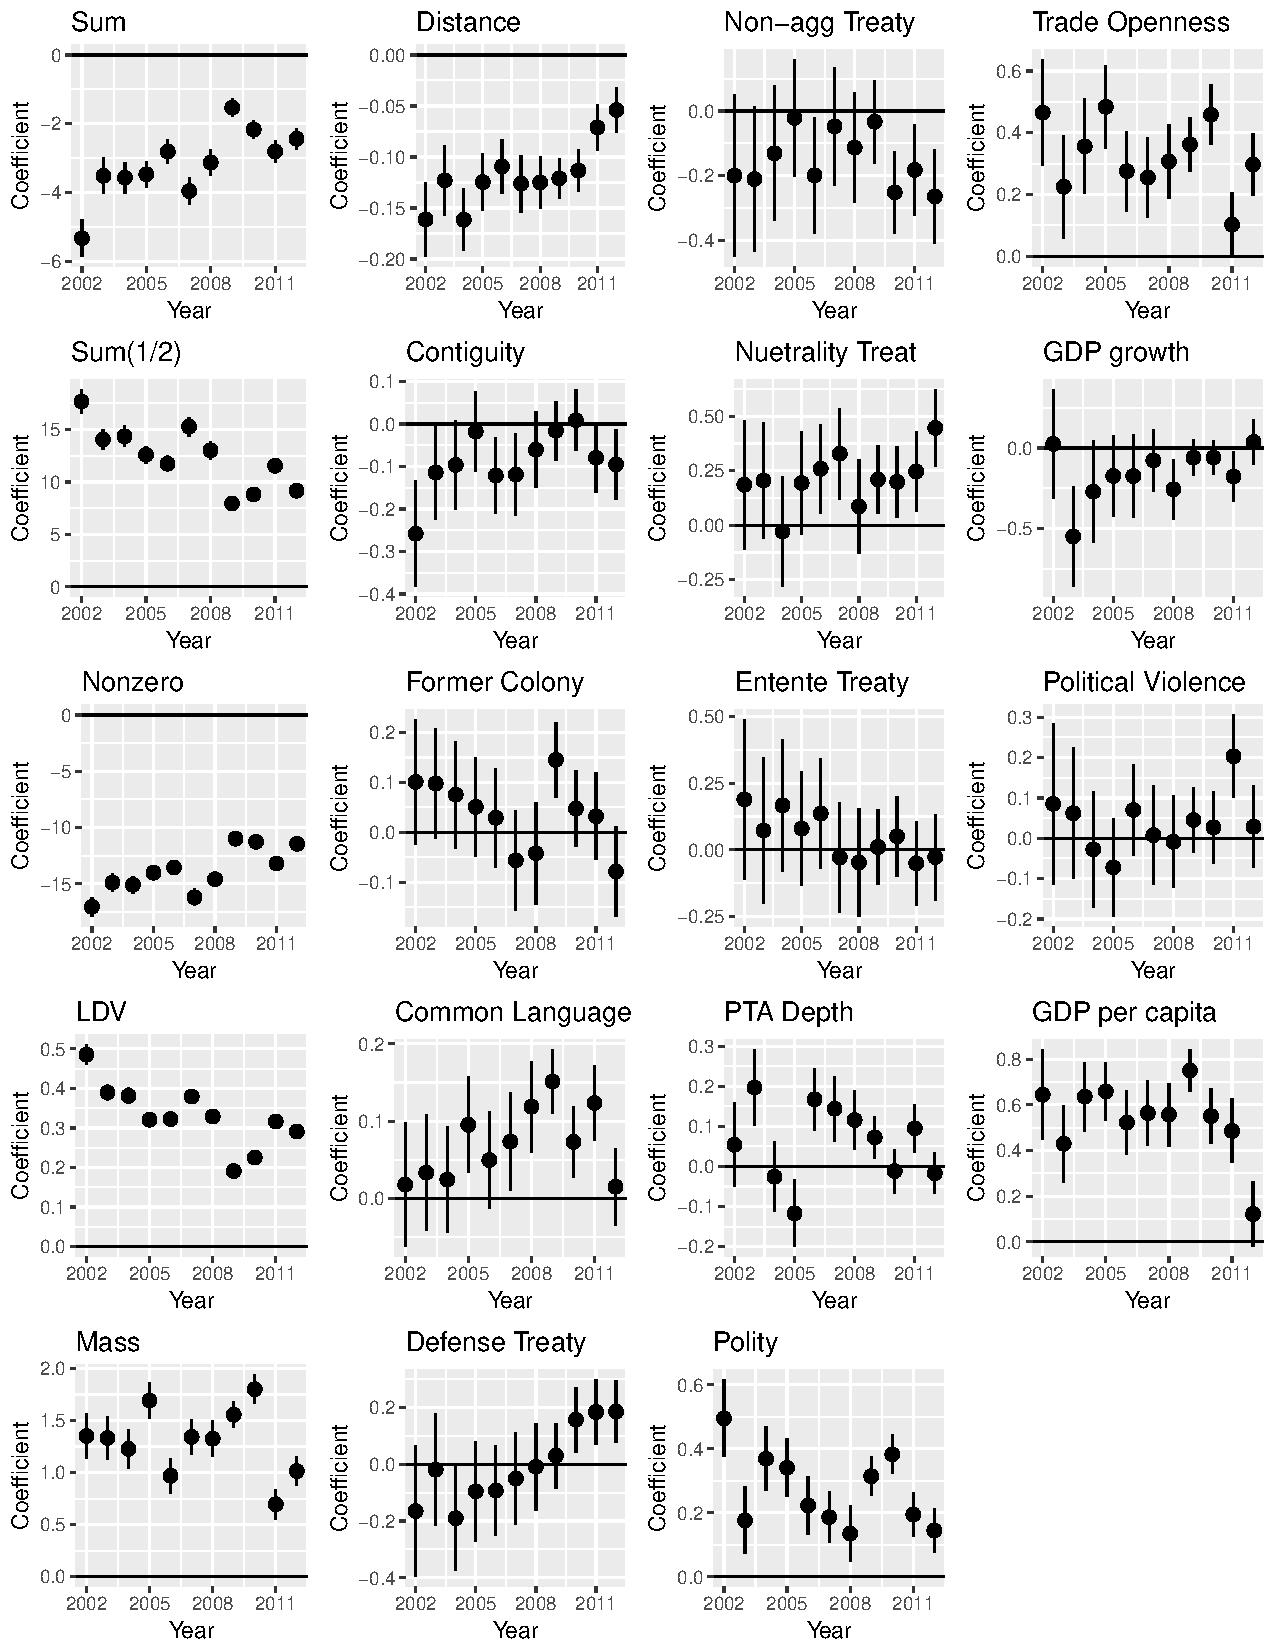
\includegraphics[scale=.75]{draft_figures/rl_plot_wo.pdf}\\
  \caption{Without Network Terms}
  \label{fig:1}
\end{figure}
\begin{figure}[h]
\centering
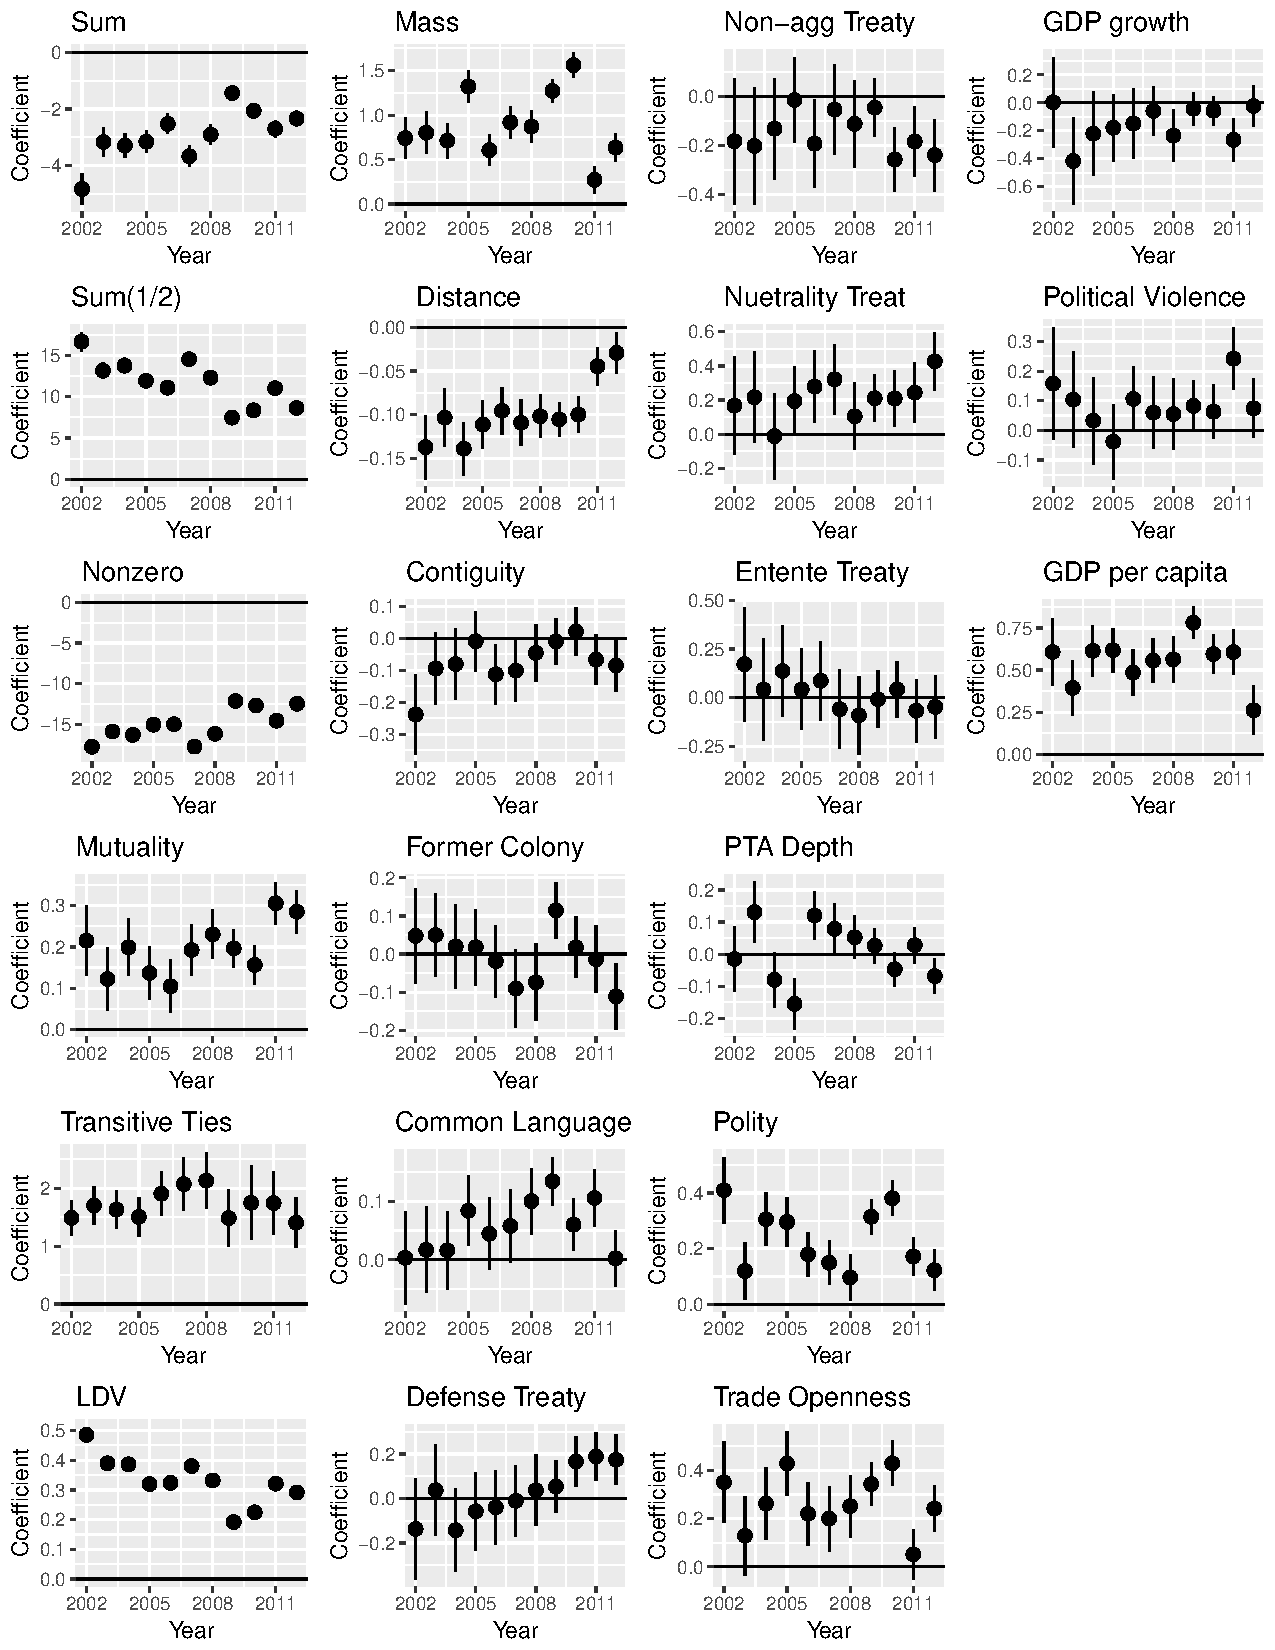
\includegraphics[scale=.75]{draft_figures/rl_plot_w.pdf}\\
  \caption{With Network Terms}
  \label{fig:1}
\end{figure}

\begin{figure}[h]
\centering
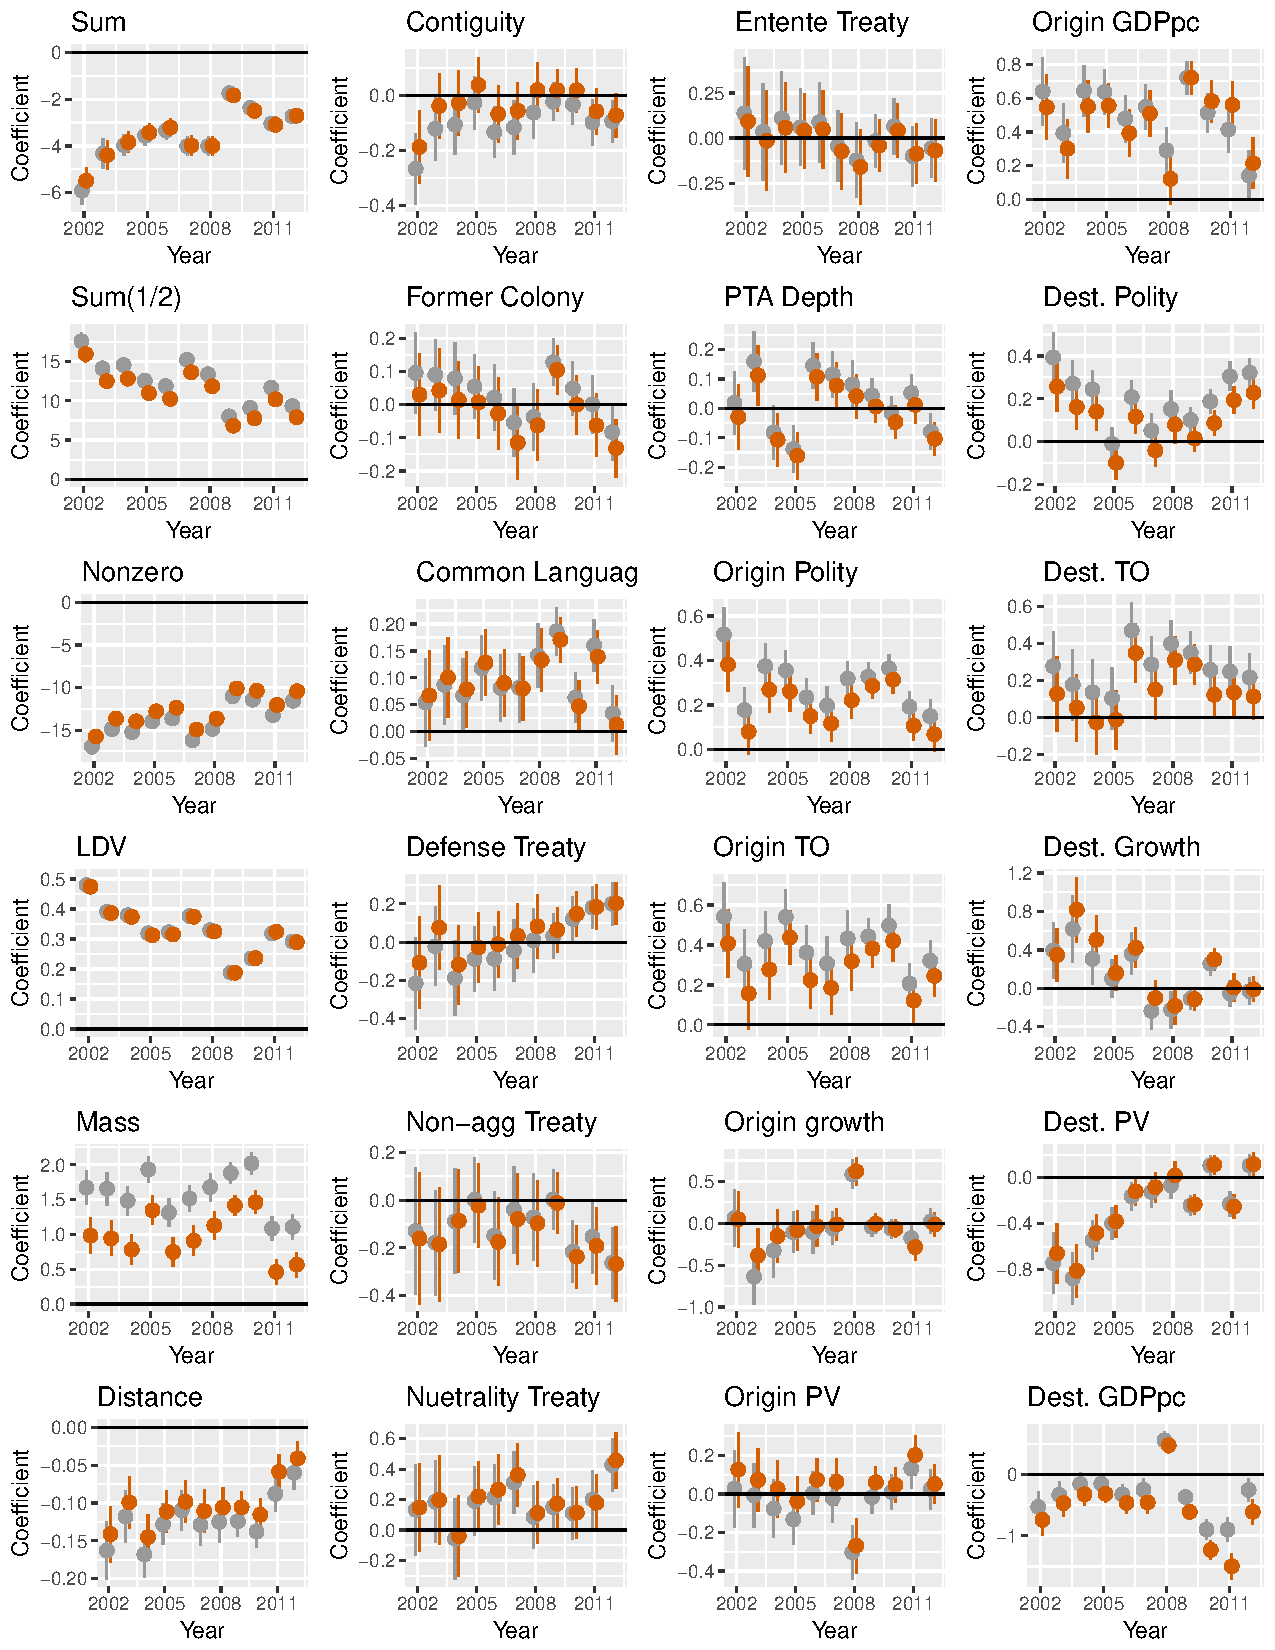
\includegraphics[scale=.75]{draft_figures/shift.pdf}\\
  \caption{Model Comparison}
  \label{fig:1}
\end{figure}

\begin{figure}[h]
\centering
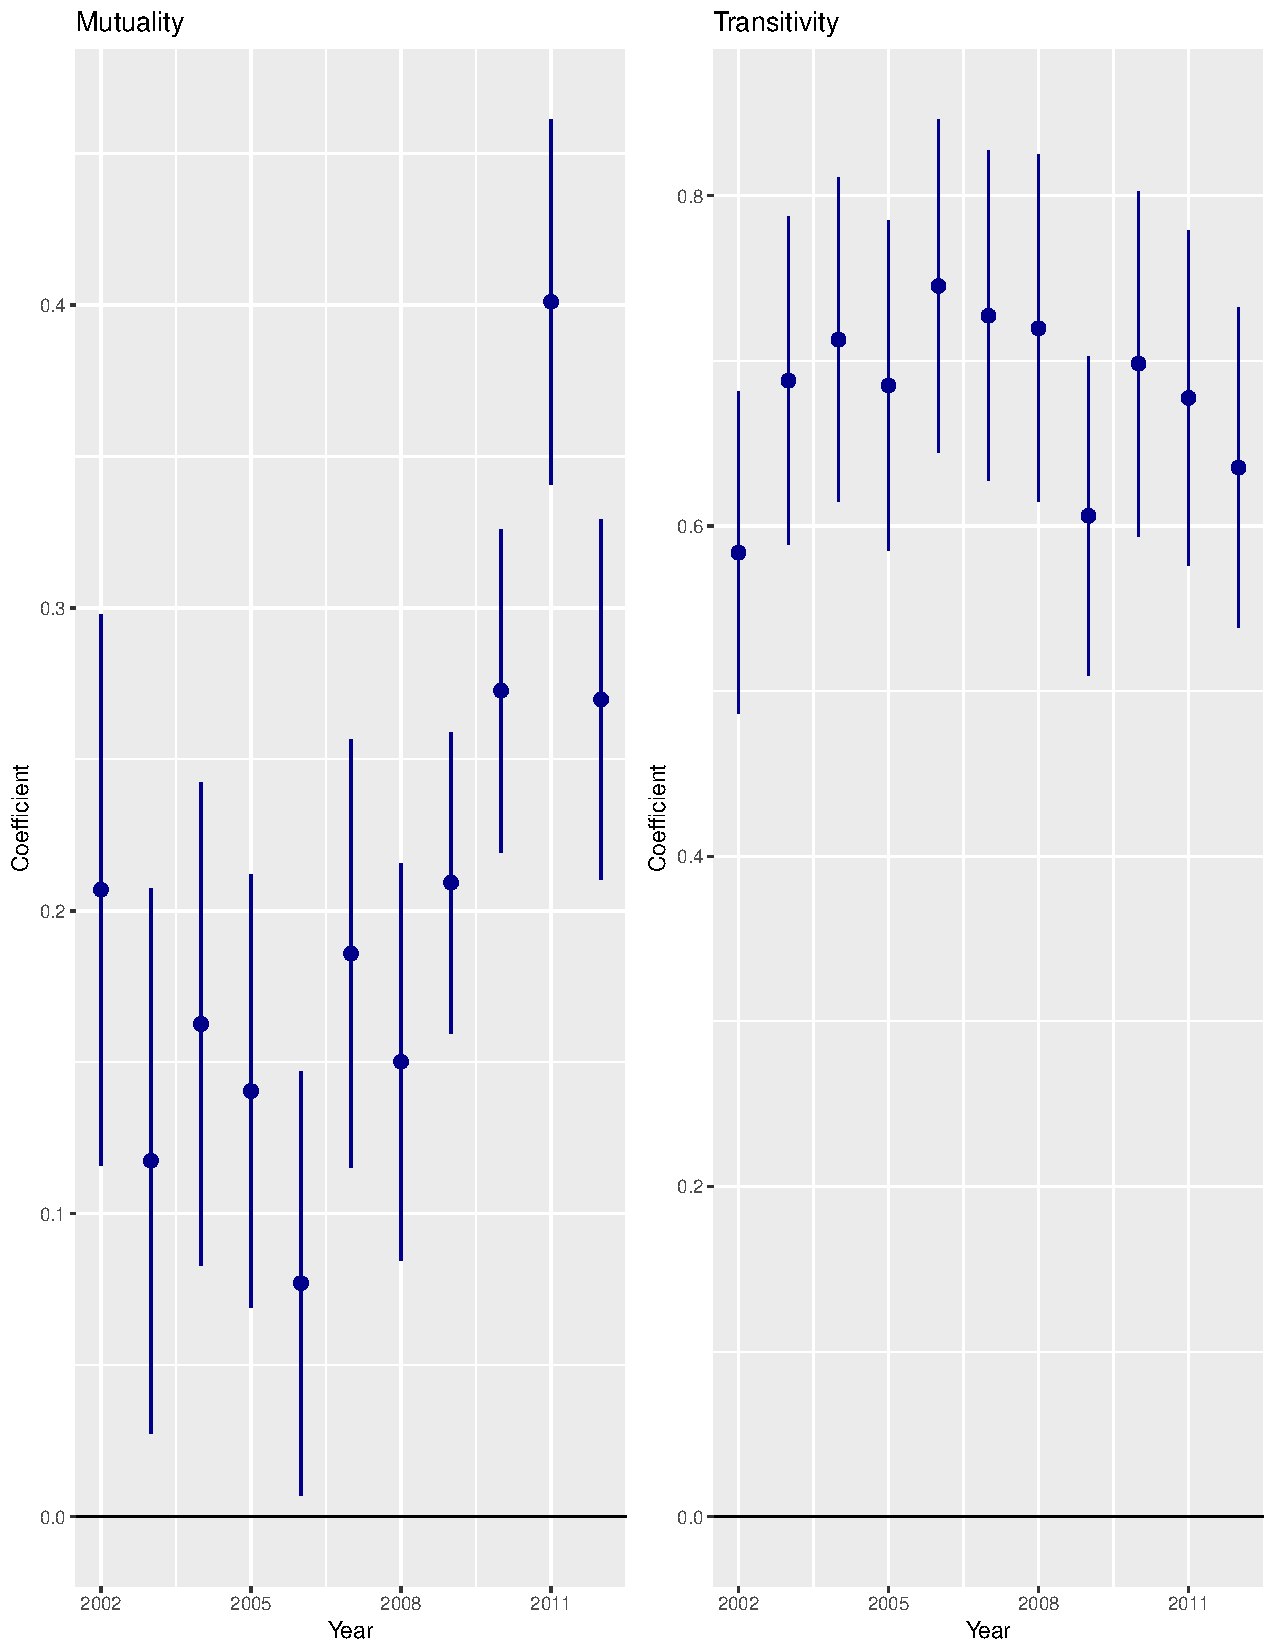
\includegraphics[scale=.75]{draft_figures/n_terms.pdf}\\
  \caption{Network Terms}
  \label{fig:1}
\end{figure}







\section{Conclusion}


\newpage
\bibliographystyle{apsr}
\bibliography{fdi_reference}


\end{document}